% =====================================================================
%  Avance 1 — Control de acceso estudiantil por código QR (TESCHA)
%  Plantilla APA 7.ª edición (clase apa7)
%  Compilar con:  latexmk -pdf trabajo.tex   (usa biber automáticamente)
% =====================================================================
\documentclass[stu,11pt,floatsintext,biblatex]{apa7}

% Fuente sans serif a 11 pt (APA permite sans serif de 11 pt, como Arial)
\usepackage{tgheros}
\renewcommand{\familydefault}{\sfdefault}

\usepackage[spanish,es-tabla]{babel} % es-tabla: "Tabla" en vez de "Cuadro"
\usepackage{csquotes}                % requerido por biblatex-apa
\addbibresource{citas.bib}

\usepackage{tikz}
\usetikzlibrary{arrows.meta,positioning,shapes.geometric}

% La clase apa7 deja el texto en bandera (raggedright) tras \maketitle;
% aquí se justifica, como pide el profesor.
\usepackage{ragged2e}
\usepackage{array}
% Columna de tabla con texto en bandera (para celdas largas).
\newcolumntype{P}[1]{>{\RaggedRight\arraybackslash}p{#1}}

% Para generar solo la sección de objetivos como PDF aparte se compila
% objetivos.tex, que define \soloobjetivos y carga este archivo.
% problema-objetivos.tex define \soloproblemaobjetivos para incluir portada,
% índice, planteamiento del problema, pregunta de investigación, objetivos,
% justificación y referencias.
% avances.tex define \soloavances para generar el informe de avances.
% justificacion.tex define \solojustificacion para generar la justificación
% como entregable aparte (introducción, impacto, viabilidad y conclusión).

% Logos arriba de la portada (los pide la escuela, no APA).
\newcommand{\hrm}{\noindent
  
\includegraphics[height=1.6cm]{img/tescha_logo.png}\hfill
  
\includegraphics[height=1.6cm]{img/logo_sitemas.png}\par}

% Índice después de la portada (lo pide la escuela; APA puro no lo usa).
\setcounter{tocdepth}{2}
\makeatletter
\patchcmd{\maketitle}{\@ifundefined{def@donotrepeattitle}}
  {\tableofcontents\newpage\@ifundefined{def@donotrepeattitle}}{}{}
% En objetivos.tex y problema-objetivos.tex no se repite el título del
% trabajo arriba del texto (equivale a la opción donotrepeattitle de apa7).
\ifdefined\soloobjetivos\def\def@donotrepeattitle{}\fi
\ifdefined\soloproblemaobjetivos\def\def@donotrepeattitle{}\fi
\patchcmd{\maketitle}{\section*{\protect\normalfont\textbf{\@title}}}
  {\section*{\protect\normalfont\textbf{\@title}}\addcontentsline{toc}{section}{\@title}}{}{}
\makeatother
\AtBeginDocument{\defbibheading{bibliography}[\refname]{%
  \clearpage\section*{\normalfont\textbf{#1}}\addcontentsline{toc}{section}{#1}}}
\newcommand{\apendiceindice}[2]{\addcontentsline{toc}{section}{\appendixname~#1: #2}}

\fancypagestyle{titlepage}{\fancyhf{}\renewcommand{\headrulewidth}{0pt}}

\renewcommand{\figurenote}[1]{\par\noindent\textit{\notelabel.} #1\par}
\renewcommand{\tablenote}[1]{\par\smallskip\figurenote{#1}}

\hypersetup{hidelinks}
\setlength{\headheight}{15.4pt}

\DeclareDelimFormat[parencite]{finalnamedelim}{\addspace\bibstring{and}\space}
\DeclareDelimFormat[bib,biblist]{finalnamedelim}{%
  \ifthenelse{\value{listcount}>\maxprtauth}{}{\addspace\bibstring{and}\space}}
\DefineBibliographyExtras{spanish}{\protected\def\bibrangedash{\textendash}}

\AtBeginDocument{%
  \renewcommand{\keywordname}{Palabras clave}%
  \renewcommand{\acksname}{Nota del autor}%
  \renewcommand{\notelabel}{Nota}%
}

% ----------------------------- Datos ---------------------------------
\ifdefined\soloavances
\title{Informe de Avances de Escanea y Entra: Control de Acceso para el TESCHA}
\else
\ifdefined\solojustificacion
\title{Justificación de Escanea y Entra: Prototipo de Acceso QR para el TESCHA}
\else
\ifdefined\soloobjetivos
\title{Objetivos de Escanea y Entra: Prototipo de Acceso QR para el TESCHA}
\else
\title{Escanea y Entra: Prototipo de Acceso QR para el TESCHA}
\fi
\fi
\fi
\shorttitle{ACCESO QR TESCHA}

\authorsnames{Juan Esteban Anzures Campos, Daniel Arellano Palacios, Ian Alexis Flores Martínez, Miguel Ángel Jurado Delgadillo, Juan Fernando Reyes Arguello, Bryan Uriel Villegas Raymundo}
\authorsaffiliations{{Ingeniería en Sistemas Computacionales, Tecnológico de Estudios Superiores de Chalco}}

% Modo stu
\course{Investigación (grupo 4751, turno vespertino)}
\ifdefined\soloavances
\professor{Docente: OMAR HETZAEL LOPEZ ALMONTE}
\duedate{13 de octubre de 2026}
\else
\professor{Dra. en C. C. Giselle Nayeli Morales Rosales}
\ifdefined\solojustificacion
\duedate{15 de octubre de 2026}
\else
\duedate{30 de septiembre de 2026}
\fi
\fi

\makeatletter
\@ifundefined{def@stu}{}{\let\@shorttitle\@undefined \let\@acks\@undefined}
\makeatother

% =====================================================================
% Nombre del plantel: la primera vez que aparece en el cuerpo de cualquier
% documento se escribe completo con su sigla; después, solo TESCHA.
% Usar siempre \tescha{} en las secciones y apéndices.
\makeatletter
\newif\iftescha@definido
\newcommand{\tescha}{\iftescha@definido TESCHA\else
  Tecnológico de Estudios Superiores de Chalco (TESCHA)%
  \global\tescha@definidotrue\fi}
\makeatother

% Casilla para opciones de la encuesta
\newcommand{\op}{\framebox[0.8em]{\rule{0pt}{0.55em}}\,}
\newcommand{\linea}[1][4cm]{\rule{#1}{0.4pt}}

\begin{document}
\maketitle
\justifying

\ifdefined\soloavances
	\widowpenalty=10000
\clubpenalty=10000
\section{Objetivo del Informe}
Presentar los avances documentales y técnicos del proyecto Escanea y Entra,
incluyendo las pruebas preliminares de reconocimiento facial, para exponer
los resultados disponibles y las actividades pendientes.

\section{Alcance del Avance}
El proyecto estudia la posibilidad de integrar un sistema de control de
acceso en el TESCHA. La propuesta de investigación se centra en códigos QR
dinámicos y en su efecto sobre el tiempo de validación y la longitud de la
fila. Durante la exploración de alternativas se desarrolló una prueba de
concepto de reconocimiento facial y se registraron intentos de calibración
con comprobación de vida.

Este informe presenta la documentación del proyecto y la evidencia de banco
disponible al 13 de octubre de 2026. Los resultados faciales permiten
examinar el funcionamiento de esa prueba de concepto. La evaluación del
acceso del TESCHA requiere todavía documentar las mediciones de campo y los
resultados del prototipo basado en QR.

También se incorpora una sesión adicional con cámara en vivo, realizada el
mismo día a las 19:04, en la que se obtuvieron capturas de localización de
rostro y detección de parpadeo. Esta evidencia visual documenta el módulo de
pose del prototipo y se presenta por separado de los 45 intentos del CSV.

\section{Avances Documentados}
Se elaboraron el planteamiento del problema, la pregunta de investigación,
los objetivos y los instrumentos de diagnóstico. El planteamiento se
presenta en texto corrido, de lo general a lo particular, con la pregunta al
final. Los objetivos específicos siguen una secuencia desde el diagnóstico
hasta la evaluación del piloto. La importancia y la viabilidad se reúnen en
la justificación del documento completo.

En el componente técnico se dispone de programas para registrar sujetos,
reconocer rostros, aplicar comprobaciones de vida y guardar los resultados
de cada intento. El registro almacena vectores por motor. El código ofrece
las opciones SFace, buffalo\_s y buffalo\_l; el CSV analizado contiene
resultados únicamente de buffalo\_l. También existe un programa que guía
sesiones por condición y otro que resume los resultados.

\begin{table}[htbp]
\caption{Estado de los Avances y su Evidencia}
\label{tab:avances-estado}
{\small\linespread{1}\selectfont
\begin{tabular}{@{}P{3.7cm}P{4.4cm}P{4.8cm}@{}}
\toprule
Componente & Avance disponible & Evidencia \\
\midrule
Documento de investigación & Planteamiento, objetivos, justificación y
metodología redactados & Documento completo y versión de planteamiento y
objetivos. \\[0.5em]
Instrumentos de diagnóstico & Encuesta, entrevista y hoja de observación
elaboradas & Apéndices A, B y C del documento completo. \\[0.5em]
Prueba de concepto facial & Registro, reconocimiento y comprobación de vida
implementados en el código & Programas de registro, reconocimiento y vida;
vectores disponibles para el código s01. \\[0.5em]
Pruebas de calibración & 45 intentos guardados y resumidos por condición &
Archivo vigente de resultados del 13 de octubre de 2026. \\[0.5em]
Comparación con QR y NFC & Resultados por documentar en la evidencia
revisada & El CSV consultado contiene registros faciales. \\[0.5em]
Evaluación en el acceso & Resultados de campo por documentar & La evidencia
consultada corresponde a pruebas de banco. \\
\bottomrule
\end{tabular}}
\tablenote{Elaboración propia a partir de los archivos del proyecto y de la
copia de evidencias del reconocimiento facial. La existencia de un
instrumento o programa se distingue de su aplicación en el acceso.}
\end{table}

\section{Pruebas Preliminares de Reconocimiento Facial}
\subsection{Modalidades y Registro}
La implementación combina el reconocimiento del rostro con una comprobación
de vida. La modalidad pasiva
evalúa un cuadro sin solicitar movimientos. La activa solicita giros,
parpadeo y retorno al frente, y comprueba que la identidad se mantenga al
final. La modalidad ambas aplica primero la comprobación pasiva y continúa
con el reto activo cuando la decisión previa permite avanzar.

La base utilizada contiene 45 intentos del 13 de octubre de 2026, registrados
entre las 16:47:56 y las 17:29:09. Se distribuyen en 20 intentos de la modalidad
ambas, 20 de la pasiva y 5 de la activa. Todos están asociados al identificador
s01 y a condiciones de calibración. La etiqueta «otras personas» no permite
determinar cuántas personas distintas participaron en esos cinco intentos.

Se tomó como fuente el archivo vigente de resultados. El respaldo contiene
20 marcas de tiempo coincidentes con este archivo, por lo que se conservó
como antecedente sin sumarlo al total. En el informe se utilizan las
etiquetas de condición y resultado esperado del archivo vigente.

\subsection{Criterios de Lectura de los Resultados}
Un intento es correcto cuando se acepta al sujeto esperado o se rechaza una
entrada etiquetada para rechazo. Un falso rechazo ocurre cuando el rostro
que debía aceptarse es rechazado. Una falsa aceptación ocurre cuando se
acepta una entrada que debía rechazarse o se acepta con una identidad
distinta de la esperada.

El campo de tiempo registra el intervalo desde que se inicia el intento con
la tecla de captura hasta que se obtiene la decisión. En la modalidad activa
incluye la respuesta de la persona al reto. La implementación inicia este
cronómetro después de obtener el cuadro inicial de la cámara, de modo que
el dato no representa el tiempo completo de llegada, colocación y cruce de
un acceso.

\subsection{Decisiones Registradas}
En conjunto se registraron 43 decisiones correctas de 45 intentos: 18 de los
20 intentos etiquetados para aceptación fueron aceptados y los 25
etiquetados para rechazo fueron rechazados. La
Tabla~\ref{tab:avances-resultados} presenta el desglose que permite
interpretar cada modalidad y condición.

\begin{table}[htbp]
\caption{Decisiones Registradas en las Pruebas de Calibración}
\label{tab:avances-resultados}
{\small\linespread{1}\selectfont
\begin{tabular}{@{}P{1.7cm}P{3.4cm}rrrr@{}}
\toprule
Modo & Condición & Intentos & Aciertos & FR & FA \\
\midrule
Ambas & Rostro real & 5 & 5/5 & 0 & 0 \\[0.5em]
Ambas & Fotografía de s01 & 10 & 10/10 & 0 & 0 \\[0.5em]
Ambas & Otras personas & 5 & 5/5 & 0 & 0 \\[0.5em]
Pasiva & Rostro real & 10 & 9/10 & 1 & 0 \\[0.5em]
Pasiva & Foto en celular & 10 & 10/10 & 0 & 0 \\[0.5em]
Activa & Rostro real & 5 & 4/5 & 1 & 0 \\[0.5em]
\bottomrule
\end{tabular}}
\tablenote{Elaboración propia a partir del CSV vigente. Todos los registros usan el motor buffalo\_l. FR = falsos rechazos; FA = falsas aceptaciones. Un acierto corresponde a aceptar la identidad esperada o rechazar un intento etiquetado para rechazo. Los intentos son repeticiones de calibración.}
\end{table}


En la modalidad pasiva se aceptó el rostro real en 9 de 10 intentos; el
rechazo restante se registró con el detalle
\texttt{pasiva\_rostro\_cortado}. En la activa hubo 4 aceptaciones de
5 intentos con rostro real; el otro se rechazó por no completar el parpadeo.
En ambas se aceptaron los 5 intentos con rostro real y se rechazaron los
10 intentos de fotografía y los 5 etiquetados como otras personas.

La modalidad pasiva también rechazó los 10 intentos con una foto en celular.
Estos resultados describen las presentaciones incluidas en el archivo. Los
casos de fotografía del modo ambas se registran como fotografía de s01, sin
especificar el soporte utilizado.

\subsection{Tiempos de Decisión}
Los tiempos medios con rostro real fueron 216,4 milisegundos para la
modalidad pasiva, 5520,6 para la activa y 6008,9 para ambas. Las dos últimas
incluyen el tiempo de realización del reto. En la modalidad ambas, los casos
rechazados antes del reto activo registraron tiempos inferiores, por lo que
conviene interpretar cada condición por separado.

\begin{table}[htbp]
\caption{Tiempos de Decisión por Condición}
\label{tab:avances-tiempos}
{\small\linespread{1}\selectfont
\begin{tabular}{@{}P{1.5cm}P{3.1cm}rrr@{}}
\toprule
Modo & Condición & Media (ms) & Mediana (ms) & Máx. (ms) \\
\midrule
Ambas & Rostro real & 6008,9 & 6494,4 & 7044,4 \\[0.5em]
Ambas & Fotografía de s01 & 245,9 & 215,2 & 300,7 \\[0.5em]
Ambas & Otras personas & 234,2 & 215,4 & 301,0 \\[0.5em]
Pasiva & Rostro real & 216,4 & 221,8 & 275,5 \\[0.5em]
Pasiva & Foto en celular & 207,1 & 218,9 & 243,5 \\[0.5em]
Activa & Rostro real & 5520,6 & 5464,2 & 7231,5 \\[0.5em]
\bottomrule
\end{tabular}}
\tablenote{Elaboración propia. Se incluyen todos los intentos de cada condición, también los rechazados. En las modalidades activa y ambas, el tiempo incluye la realización del reto. En ambas, un rechazo previo puede detener el proceso sin ejecutar el reto activo.}
\end{table}


\clearpage
\begin{figure}[!ht]
\caption{Tiempo Medio de Decisión en los Intentos con Rostro Real}
\label{fig:avances-tiempos}
\centering
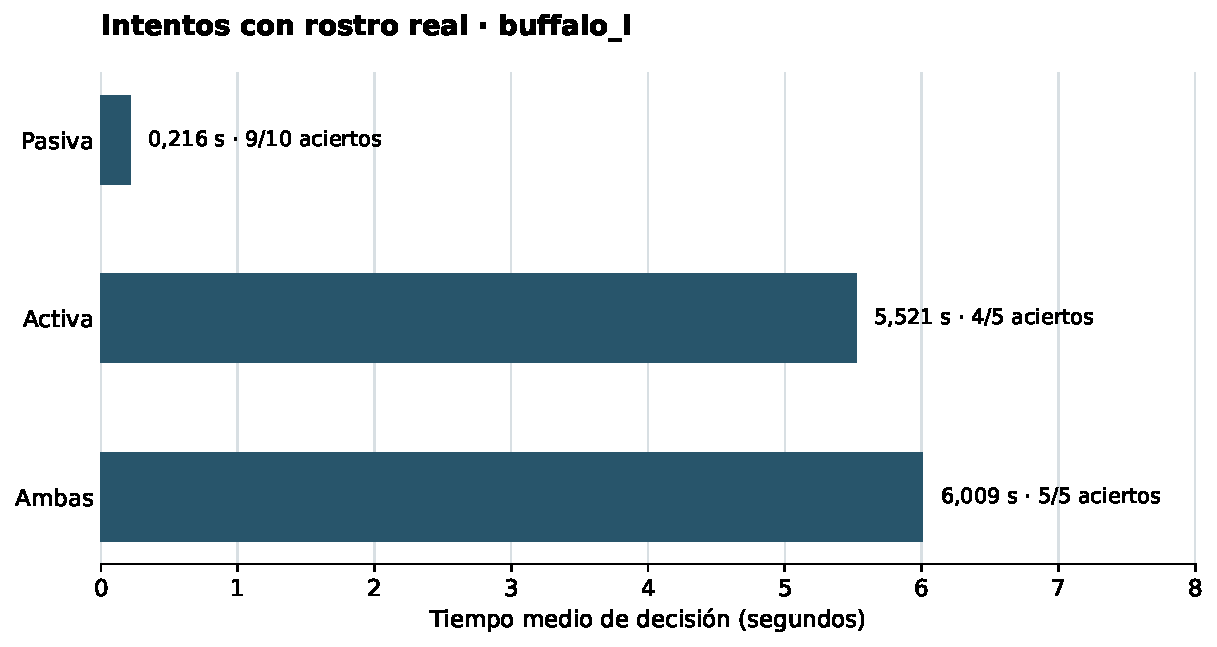
\includegraphics[width=0.96\linewidth]{evidencias/avances-2026-10-13/tiempos-rostro-real.pdf}
\figurenote{Elaboración propia con el CSV vigente. Las etiquetas indican
tiempo medio y aciertos por intentos. Se incluyen los rechazos en los
promedios. Activa y ambas incorporan la duración del reto; las condiciones
son de calibración y tienen distinto número de repeticiones.}
\end{figure}

\section{Interpretación del Avance}
La evidencia muestra que se dispone de un proceso que registra sujetos,
realiza reconocimiento y comprobación de vida y guarda decisiones y tiempos.
También permitió identificar dos situaciones para revisar: el encuadre del
rostro durante la comprobación pasiva y la ejecución del parpadeo en el reto
activo. Esos hallazgos orientan ajustes de uso y nuevas pruebas.

Los 45 intentos son repeticiones de calibración asociadas a un mismo código,
con grupos pequeños y desiguales. Los aciertos observados describen esta
sesión; todavía se requieren sesiones con más participantes y condiciones
registradas para estimar el desempeño en la población del TESCHA.

El archivo no conserva por intento el equipo de cómputo, la fuente de
cámara, las condiciones de iluminación ni la versión y configuración
exactas del programa. Las opciones descritas en este informe proceden del
código disponible al realizar la copia. Esta información deberá acompañar
las siguientes sesiones para facilitar su reproducción.

En los registros analizados no aparecen ensayos de QR, NFC, SFace,
buffalo\_s o reconocimiento sin comprobación de vida. Para comparar tiempos
entre tecnologías será necesario medir el mismo recorrido de validación.
La interpretación del efecto en la fila requiere además datos del acceso.

\section{Próximas Actividades}
\begin{itemize}
\interlinepenalty=10000
\item Registrar el equipo, la cámara, la configuración y las condiciones de
cada sesión antes de ampliar las pruebas.
\item Revisar el encuadre y las instrucciones del reto a partir de los dos
falsos rechazos observados.
\item Ampliar los participantes y completar las condiciones previstas de
iluminación y presentación de fotografías con identificación clara de cada caso.
\item Obtener pruebas comparables de QR y NFC con un criterio común de
inicio y fin de la validación.
\item Documentar la integración del prototipo de acceso y las mediciones de
campo necesarias para evaluar su efecto en el TESCHA.
\end{itemize}

\section{Evidencias del Informe}
La evidencia numérica procede de la carpeta de reconocimiento facial
proporcionada por el equipo. La copia conservada en
\path{evidencias/avances-2026-10-13/} contiene el CSV vigente, su respaldo,
la documentación, los programas y el resumen utilizado para las tablas y la
gráfica. El registro de procedencia identifica los archivos empleados.

Las capturas reales de la sesión adicional se conservan en la subcarpeta
\path{camara/}. Su registro incluye la fecha, el evento detectado y las
dimensiones de cada cuadro. Esta sesión utiliza el módulo de pose del
prototipo y documenta la localización del rostro y el parpadeo.

\clearpage
\section{Evidencia Visual de las Pruebas}
Las siguientes imágenes se obtuvieron de la cámara durante una sesión con
un participante voluntario. La primera documenta la localización del rostro
y la segunda el parpadeo detectado por el módulo de pose.

\begin{figure}[!ht]
\caption{Captura de la Prueba de Localización del Rostro}
\label{fig:avances-camara-deteccion}
\centering
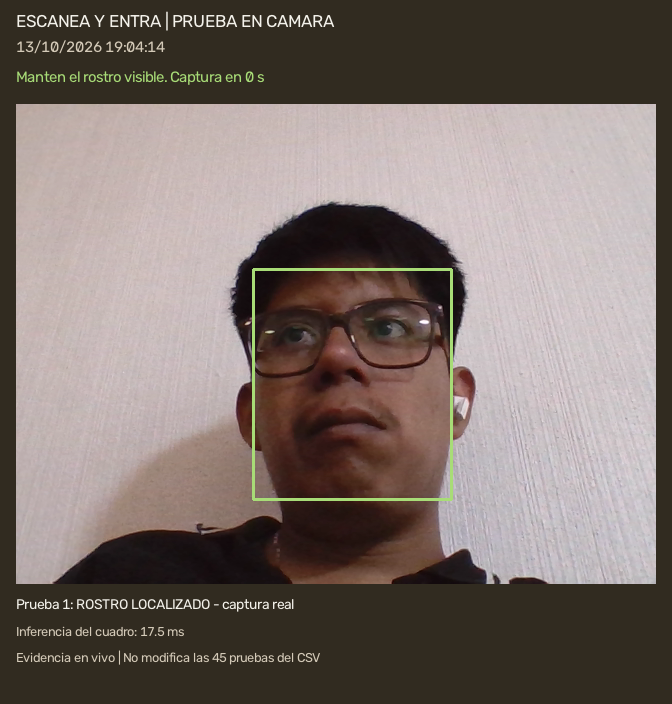
\includegraphics[width=0.85\linewidth]{evidencias/avances-2026-10-13/camara/01-deteccion.png}
\figurenote{Captura real del 13 de octubre de 2026 a las 19:04:14. El recuadro
indica el rostro localizado. El tiempo mostrado corresponde al procesamiento
de ese cuadro.}
\end{figure}

\clearpage
\begin{figure}[!ht]
\caption{Captura de la Prueba de Detección de Parpadeo}
\label{fig:avances-camara-parpadeo}
\centering
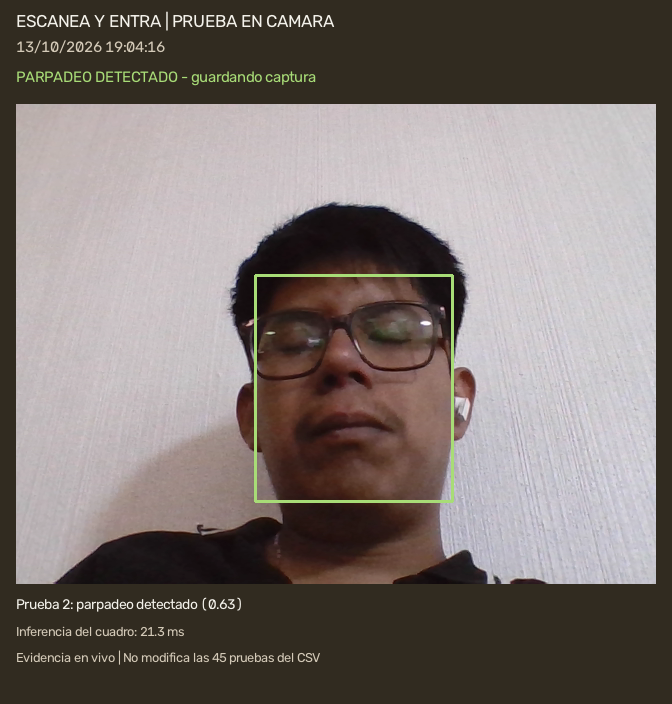
\includegraphics[width=0.85\linewidth]{evidencias/avances-2026-10-13/camara/02-parpadeo.png}
\figurenote{Captura real del 13 de octubre de 2026 a las 19:04:16. El módulo
registró una puntuación de parpadeo de 0,63, superior al umbral de 0,50
utilizado en esta prueba. La sesión adicional documenta detección y movimiento;
el resumen estadístico corresponde a los 45 intentos del archivo original.}
\end{figure}

\else
	\ifdefined\solojustificacion
		% Justificación como entregable aparte (justificacion.tex).
% Sigue el material de clase de Taller de Investigación I (TecNM): impacto
% social, tecnológico, económico y ético, y viabilidad. Se omite el impacto
% ambiental porque el proyecto no tiene una relación directa con el ambiente
% ni con el uso de recursos naturales.
% La justificación no lleva introducción ni tablas (las retiradas están en
% tablas/). La viabilidad está en secciones/12-viabilidad.tex.
% Redacción en tercera persona.
% Los antecedentes (estudios previos) están en secciones/11-antecedentes.tex.
%
% En justificacion.tex los apartados son secciones; dentro de otro documento
% (problema-objetivos.tex) quedan como subsecciones de «Justificación».
\ifdefined\solojustificacion
\let\justsec\section
\let\justsubsec\subsection
\else
\section{Justificación}
\let\justsec\subsection
\let\justsubsec\subsubsection
\fi

\justsec{Impacto}

\justsubsec{Impacto Social}
La investigación puede beneficiar, en primer lugar, a los estudiantes, que
pierden tiempo en las filas de entrada y se exponen a llegar tarde a su
primera clase. Medir el tiempo de validación y la longitud de la fila antes
y durante el piloto permitirá saber si un cambio en el mecanismo de acceso
alivia esa situación o si la espera se debe a otras causas.

También puede beneficiar al personal de vigilancia, que revisa cientos de
credenciales en pocos minutos y cuya revisión depende solo de su atención en
los momentos de mayor afluencia. Por último, el Departamento de Control
Escolar y los directivos contarían con datos de ingreso por franja horaria
que hoy no existen, útiles para planear la apertura de accesos y el personal
necesario en cada horario. Como información complementaria, el registro de
intentos rechazados aportaría una primera medida de la presentación de
credenciales ajenas o vencidas, una preocupación de seguridad cuya magnitud
tampoco se conoce.

\justsubsec{Impacto Tecnológico}
Desde la dimensión tecnológica, el proyecto integra componentes de hardware
y software en un mismo sistema: un microcontrolador con cámara que captura y
decodifica el código, un controlador que libera el torniquete, un servidor
que valida el código y una base de datos con un panel web para consultar los
registros.

La evidencia disponible sobre el ESP32-CAM aborda la transmisión de video y
no la decodificación de códigos QR \parencite{nowroz2025esp32cam}. Las
pruebas del prototipo bajo distintas condiciones de iluminación, brillo de
pantalla y distancia permitirán conocer su tiempo de lectura y su tasa de
lecturas fallidas. Estos resultados, junto con la documentación del diseño,
podrán servir como precedente para otros proyectos del \tescha{} que
busquen automatizar procesos con componentes de bajo costo.

\justsubsec{Impacto Económico}
El sistema se apoya en el celular que ya posee el estudiante, por lo que no
es necesario emitir tarjetas ni credenciales adicionales, y el lector se
construye con componentes de bajo costo. Frente a otras tecnologías de
validación, como NFC o el reconocimiento facial, el código QR requiere menos
infraestructura. Sin embargo, cualquier ahorro en tiempo de trabajo del
personal o en costos de operación tendría que comprobarse en evaluaciones
posteriores; esta investigación solo aportará la información del piloto para
valorarlo.

\justsubsec{Impacto Ético}
El sistema trata datos personales de los estudiantes, como su identidad y
la hora de ingreso. Por ello, antes del piloto se identificarán los
requisitos de la legislación estatal \parencite{edomex2017datos} y general
\parencite{lgpdppso2025}, y se definirán con Control Escolar el aviso de
privacidad y el resguardo de los registros. A diferencia del reconocimiento
facial, el código QR no trata datos biométricos, y quien no pueda mostrar su
código seguirá el procedimiento manual actual.

% La viabilidad pasará al documento de metodología; solo el entregable
% justificacion.tex la conserva.
\ifdefined\solojustificacion
% Viabilidad del proyecto. Se retiró de la justificación de
% problema-objetivos.tex porque irá en el documento de metodología (aún no
% existe). Por ahora solo la carga justificacion.tex.
% Redacción en tercera persona.
\ifdefined\justsec\justsec{Viabilidad}\else\section{Viabilidad}\fi
El proyecto propone construir un prototipo de torniquete con un lector
ESP32-CAM que valide un código QR dinámico mostrado en el celular del
estudiante y registre cada ingreso en una base de datos consultable desde
un panel web. El prototipo se probará en un acceso peatonal piloto del
turno vespertino para evaluar su efecto en el tiempo de validación y en la
longitud de la fila.

La viabilidad técnica se sustenta en que los componentes del prototipo, el
ESP32-CAM, el controlador del torniquete, el servidor y la base de datos,
están disponibles comercialmente y corresponden a conocimientos que se han
adquirido en Ingeniería en Sistemas Computacionales. Ya se ha trabajado con
captura de imágenes en pruebas de banco durante la exploración de
alternativas, lo que reduce el riesgo de la etapa de desarrollo. Frente a
NFC, una comparación en transacciones móviles encontró que el QR se procesa
con mayor rapidez, aunque no incorpora cifrado propio
\parencite{harnaningrum2024comparison}; esa carencia se compensa con la firma
HMAC del código.

En cuanto a los recursos económicos, el bajo costo de los componentes
permite construir y probar el prototipo con recursos propios, sin depender
de una inversión institucional. En cuanto al tiempo, el trabajo se organiza
en cinco fases (diagnóstico, diseño de hardware y firmware, desarrollo del
servidor, piloto controlado y evaluación), y el estudio se limita a un solo
acceso peatonal y a la franja de mayor afluencia del turno vespertino, lo
que lo hace abarcable en el periodo escolar.

El acceso a la información y a los participantes es posible porque el
proyecto se desarrolla dentro del \tescha{}: se puede observar el acceso
piloto y aplicar la encuesta a estudiantes y las entrevistas al personal de
vigilancia y de Control Escolar. La instalación del prototipo en el acceso
requiere la autorización de las autoridades del plantel, que se solicitará
antes del piloto.

Queda por confirmar la viabilidad desde el lado del estudiante, es decir, si
cuenta con un celular propio, con conexión a internet y con batería
suficiente al llegar al plantel. Esta condición se indagará con la encuesta
del diagnóstico, y sus resultados indicarán si el sistema puede usarse de
forma general o si el procedimiento manual debe mantenerse para una parte de
los estudiantes.

\fi

\justsec{Conclusión}
Hoy no existen datos que midan el problema del acceso en el \tescha{}: se
desconoce cuánto tiempo espera un estudiante para entrar y qué longitud
alcanzan las filas. La investigación se justifica porque puede generar esa
información y contrastarla con el desempeño de un prototipo de bajo costo.

En conjunto, los resultados podrán aportar evidencia del propio plantel para
valorar si un sistema de acceso con códigos QR dinámicos ayuda a aliviar
las esperas del sistema actual y si conviene ampliar el piloto a otros
accesos. No obstante, esa posible ampliación y sus beneficios económicos
tendrían que confirmarse mediante evaluaciones posteriores.


		\printbibliography
	\else
		\ifdefined\soloobjetivos
			\section{Planteamiento del Problema}
El control de acceso en las instituciones educativas permite regular el
ingreso de estudiantes y disponer de información sobre la entrada de personas
al plantel. Cuando este proceso depende de la revisión visual de credenciales
o de registros manuales, la atención está condicionada por la capacidad del
personal encargado y por la cantidad de personas que llegan al mismo tiempo.
La concentración de estudiantes antes del inicio de clases puede dificultar
la fluidez del acceso y la disponibilidad de un registro de ingresos.

Entre las alternativas tecnológicas para apoyar este proceso se encuentran
los sistemas basados en códigos QR, cuyo uso para el control de acceso físico
se ha propuesto en la literatura \parencite{kao2011physical}. Su incorporación
en un plantel requiere conocer las condiciones del acceso y el efecto que
podría tener en su funcionamiento. La disponibilidad de una tecnología, por
sí sola, no permite establecer cómo responderá a las necesidades de una
institución determinada.

En el \tescha{}, el ingreso de los
estudiantes se controla mediante la revisión visual de credenciales físicas
por parte del personal de vigilancia. En los minutos previos al inicio de
clases del turno vespertino se concentra la llegada de estudiantes y se
presentan filas en los accesos peatonales. Además, el procedimiento actual
no genera un registro digital de quién ingresa ni de la hora de entrada.

La situación plantea dificultades para atender el flujo de estudiantes y
conocer el funcionamiento del acceso. Sin embargo, no se dispone de
mediciones suficientes para precisar el tiempo que requiere la validación
de cada estudiante ni la longitud que alcanzan las filas. La posible
presentación de credenciales ajenas constituye una preocupación
complementaria relacionada con la seguridad, cuya magnitud tampoco se ha
establecido.

El problema de investigación se centra en el desconocimiento del efecto que
un sistema de acceso con códigos QR dinámicos tendría en estas condiciones.
En particular, se desconoce si su incorporación modificaría el tiempo de
validación y la longitud de la fila en el acceso peatonal del \tescha{}. Esta
falta de información limita la posibilidad de valorar su integración en el
plantel a partir de evidencia del propio contexto.

El estudio se delimita al acceso peatonal piloto del turno vespertino y al
proceso de ingreso de los estudiantes al plantel. A partir de esta situación,
se plantea la siguiente pregunta de investigación:
¿Cuál es el efecto de implementar un sistema automatizado de
validación mediante códigos QR dinámicos en la eficiencia general del control
de acceso peatonal de los estudiantes del TESCHA?



			\section{Objetivos}

\subsection{Objetivo General}
Evaluar el efecto de un prototipo con códigos QR dinámicos en el
control de acceso peatonal del \tescha{} para valorar la posibilidad de
integrar este sistema en el plantel.

\subsection{Objetivos Específicos}
\begin{itemize}
	\item Analizar la situación actual del acceso mediante observación,
	      encuestas y entrevistas para establecer una línea base del flujo,
	      el tiempo de validación y la fila, registrando las incidencias de
	      identidad como información complementaria.
	\item Estimar la viabilidad del sistema desde el lado del estudiante
	      mediante una encuesta sobre la disponibilidad de celular, conexión
	      y batería al llegar al plantel.
	\item Identificar los requisitos de protección de datos personales del
	      sistema, revisando la normativa aplicable y consultando a Control
	      Escolar.
	\item Diseñar la arquitectura del sistema, integrando el lector,
	      el torniquete, el servidor, la base de datos y el panel web para
	      registrar los ingresos.
	\item Implementar la generación y validación de códigos QR dinámicos
	      firmados con HMAC, verificando el rechazo de códigos
	      vencidos, repetidos o alterados y la tolerancia a desfases de reloj
	      antes de integrar los componentes del prototipo.
	\item Construir un prototipo funcional que integre la lectura del
	      QR, la apertura del torniquete y el registro y consulta de ingresos
	      para realizar el piloto.
	\item Verificar el desempeño técnico del prototipo, midiendo el
	      tiempo de lectura y validación y la tasa de lecturas fallidas bajo
	      distintas condiciones de iluminación, brillo y distancia antes
	      del piloto.
	\item Evaluar el efecto del prototipo en el tiempo de validación
	      y la longitud de la fila, comparando la línea base con el piloto
	      para valorar su posible integración en el control de acceso.
\end{itemize}

% La relación con la pregunta solo aparece en el documento completo.
\ifdefined\soloproblemaobjetivos\else\ifdefined\soloobjetivos\else
\subsection{Relación con la Pregunta de Investigación}
Los objetivos abarcan el diagnóstico del acceso, la definición de requisitos,
el desarrollo del prototipo y su evaluación. La comparación con la línea base
permite responder la pregunta mediante el tiempo de validación y la longitud
de la fila. Las incidencias de identidad se registran como información
complementaria sobre seguridad.
\fi\fi


			\clearpage
			% Justificación como entregable aparte (justificacion.tex).
% Sigue el material de clase de Taller de Investigación I (TecNM): impacto
% social, tecnológico, económico y ético, y viabilidad. Se omite el impacto
% ambiental porque el proyecto no tiene una relación directa con el ambiente
% ni con el uso de recursos naturales.
% La justificación no lleva introducción ni tablas (las retiradas están en
% tablas/). La viabilidad está en secciones/12-viabilidad.tex.
% Redacción en tercera persona.
% Los antecedentes (estudios previos) están en secciones/11-antecedentes.tex.
%
% En justificacion.tex los apartados son secciones; dentro de otro documento
% (problema-objetivos.tex) quedan como subsecciones de «Justificación».
\ifdefined\solojustificacion
\let\justsec\section
\let\justsubsec\subsection
\else
\section{Justificación}
\let\justsec\subsection
\let\justsubsec\subsubsection
\fi

\justsec{Impacto}

\justsubsec{Impacto Social}
La investigación puede beneficiar, en primer lugar, a los estudiantes, que
pierden tiempo en las filas de entrada y se exponen a llegar tarde a su
primera clase. Medir el tiempo de validación y la longitud de la fila antes
y durante el piloto permitirá saber si un cambio en el mecanismo de acceso
alivia esa situación o si la espera se debe a otras causas.

También puede beneficiar al personal de vigilancia, que revisa cientos de
credenciales en pocos minutos y cuya revisión depende solo de su atención en
los momentos de mayor afluencia. Por último, el Departamento de Control
Escolar y los directivos contarían con datos de ingreso por franja horaria
que hoy no existen, útiles para planear la apertura de accesos y el personal
necesario en cada horario. Como información complementaria, el registro de
intentos rechazados aportaría una primera medida de la presentación de
credenciales ajenas o vencidas, una preocupación de seguridad cuya magnitud
tampoco se conoce.

\justsubsec{Impacto Tecnológico}
Desde la dimensión tecnológica, el proyecto integra componentes de hardware
y software en un mismo sistema: un microcontrolador con cámara que captura y
decodifica el código, un controlador que libera el torniquete, un servidor
que valida el código y una base de datos con un panel web para consultar los
registros.

La evidencia disponible sobre el ESP32-CAM aborda la transmisión de video y
no la decodificación de códigos QR \parencite{nowroz2025esp32cam}. Las
pruebas del prototipo bajo distintas condiciones de iluminación, brillo de
pantalla y distancia permitirán conocer su tiempo de lectura y su tasa de
lecturas fallidas. Estos resultados, junto con la documentación del diseño,
podrán servir como precedente para otros proyectos del \tescha{} que
busquen automatizar procesos con componentes de bajo costo.

\justsubsec{Impacto Económico}
El sistema se apoya en el celular que ya posee el estudiante, por lo que no
es necesario emitir tarjetas ni credenciales adicionales, y el lector se
construye con componentes de bajo costo. Frente a otras tecnologías de
validación, como NFC o el reconocimiento facial, el código QR requiere menos
infraestructura. Sin embargo, cualquier ahorro en tiempo de trabajo del
personal o en costos de operación tendría que comprobarse en evaluaciones
posteriores; esta investigación solo aportará la información del piloto para
valorarlo.

\justsubsec{Impacto Ético}
El sistema trata datos personales de los estudiantes, como su identidad y
la hora de ingreso. Por ello, antes del piloto se identificarán los
requisitos de la legislación estatal \parencite{edomex2017datos} y general
\parencite{lgpdppso2025}, y se definirán con Control Escolar el aviso de
privacidad y el resguardo de los registros. A diferencia del reconocimiento
facial, el código QR no trata datos biométricos, y quien no pueda mostrar su
código seguirá el procedimiento manual actual.

% La viabilidad pasará al documento de metodología; solo el entregable
% justificacion.tex la conserva.
\ifdefined\solojustificacion
% Viabilidad del proyecto. Se retiró de la justificación de
% problema-objetivos.tex porque irá en el documento de metodología (aún no
% existe). Por ahora solo la carga justificacion.tex.
% Redacción en tercera persona.
\ifdefined\justsec\justsec{Viabilidad}\else\section{Viabilidad}\fi
El proyecto propone construir un prototipo de torniquete con un lector
ESP32-CAM que valide un código QR dinámico mostrado en el celular del
estudiante y registre cada ingreso en una base de datos consultable desde
un panel web. El prototipo se probará en un acceso peatonal piloto del
turno vespertino para evaluar su efecto en el tiempo de validación y en la
longitud de la fila.

La viabilidad técnica se sustenta en que los componentes del prototipo, el
ESP32-CAM, el controlador del torniquete, el servidor y la base de datos,
están disponibles comercialmente y corresponden a conocimientos que se han
adquirido en Ingeniería en Sistemas Computacionales. Ya se ha trabajado con
captura de imágenes en pruebas de banco durante la exploración de
alternativas, lo que reduce el riesgo de la etapa de desarrollo. Frente a
NFC, una comparación en transacciones móviles encontró que el QR se procesa
con mayor rapidez, aunque no incorpora cifrado propio
\parencite{harnaningrum2024comparison}; esa carencia se compensa con la firma
HMAC del código.

En cuanto a los recursos económicos, el bajo costo de los componentes
permite construir y probar el prototipo con recursos propios, sin depender
de una inversión institucional. En cuanto al tiempo, el trabajo se organiza
en cinco fases (diagnóstico, diseño de hardware y firmware, desarrollo del
servidor, piloto controlado y evaluación), y el estudio se limita a un solo
acceso peatonal y a la franja de mayor afluencia del turno vespertino, lo
que lo hace abarcable en el periodo escolar.

El acceso a la información y a los participantes es posible porque el
proyecto se desarrolla dentro del \tescha{}: se puede observar el acceso
piloto y aplicar la encuesta a estudiantes y las entrevistas al personal de
vigilancia y de Control Escolar. La instalación del prototipo en el acceso
requiere la autorización de las autoridades del plantel, que se solicitará
antes del piloto.

Queda por confirmar la viabilidad desde el lado del estudiante, es decir, si
cuenta con un celular propio, con conexión a internet y con batería
suficiente al llegar al plantel. Esta condición se indagará con la encuesta
del diagnóstico, y sus resultados indicarán si el sistema puede usarse de
forma general o si el procedimiento manual debe mantenerse para una parte de
los estudiantes.

\fi

\justsec{Conclusión}
Hoy no existen datos que midan el problema del acceso en el \tescha{}: se
desconoce cuánto tiempo espera un estudiante para entrar y qué longitud
alcanzan las filas. La investigación se justifica porque puede generar esa
información y contrastarla con el desempeño de un prototipo de bajo costo.

En conjunto, los resultados podrán aportar evidencia del propio plantel para
valorar si un sistema de acceso con códigos QR dinámicos ayuda a aliviar
las esperas del sistema actual y si conviene ampliar el piloto a otros
accesos. No obstante, esa posible ampliación y sus beneficios económicos
tendrían que confirmarse mediante evaluaciones posteriores.


			\printbibliography
		\else
			\ifdefined\soloproblemaobjetivos
				\section{Planteamiento del Problema}
El control de acceso en las instituciones educativas permite regular el
ingreso de estudiantes y disponer de información sobre la entrada de personas
al plantel. Cuando este proceso depende de la revisión visual de credenciales
o de registros manuales, la atención está condicionada por la capacidad del
personal encargado y por la cantidad de personas que llegan al mismo tiempo.
La concentración de estudiantes antes del inicio de clases puede dificultar
la fluidez del acceso y la disponibilidad de un registro de ingresos.

Entre las alternativas tecnológicas para apoyar este proceso se encuentran
los sistemas basados en códigos QR, cuyo uso para el control de acceso físico
se ha propuesto en la literatura \parencite{kao2011physical}. Su incorporación
en un plantel requiere conocer las condiciones del acceso y el efecto que
podría tener en su funcionamiento. La disponibilidad de una tecnología, por
sí sola, no permite establecer cómo responderá a las necesidades de una
institución determinada.

En el \tescha{}, el ingreso de los
estudiantes se controla mediante la revisión visual de credenciales físicas
por parte del personal de vigilancia. En los minutos previos al inicio de
clases del turno vespertino se concentra la llegada de estudiantes y se
presentan filas en los accesos peatonales. Además, el procedimiento actual
no genera un registro digital de quién ingresa ni de la hora de entrada.

La situación plantea dificultades para atender el flujo de estudiantes y
conocer el funcionamiento del acceso. Sin embargo, no se dispone de
mediciones suficientes para precisar el tiempo que requiere la validación
de cada estudiante ni la longitud que alcanzan las filas. La posible
presentación de credenciales ajenas constituye una preocupación
complementaria relacionada con la seguridad, cuya magnitud tampoco se ha
establecido.

El problema de investigación se centra en el desconocimiento del efecto que
un sistema de acceso con códigos QR dinámicos tendría en estas condiciones.
En particular, se desconoce si su incorporación modificaría el tiempo de
validación y la longitud de la fila en el acceso peatonal del \tescha{}. Esta
falta de información limita la posibilidad de valorar su integración en el
plantel a partir de evidencia del propio contexto.

El estudio se delimita al acceso peatonal piloto del turno vespertino y al
proceso de ingreso de los estudiantes al plantel. A partir de esta situación,
se plantea la siguiente pregunta de investigación:
¿Cuál es el efecto de implementar un sistema automatizado de
validación mediante códigos QR dinámicos en la eficiencia general del control
de acceso peatonal de los estudiantes del TESCHA?



				\section{Objetivos}

\subsection{Objetivo General}
Evaluar el efecto de un prototipo con códigos QR dinámicos en el
control de acceso peatonal del \tescha{} para valorar la posibilidad de
integrar este sistema en el plantel.

\subsection{Objetivos Específicos}
\begin{itemize}
	\item Analizar la situación actual del acceso mediante observación,
	      encuestas y entrevistas para establecer una línea base del flujo,
	      el tiempo de validación y la fila, registrando las incidencias de
	      identidad como información complementaria.
	\item Estimar la viabilidad del sistema desde el lado del estudiante
	      mediante una encuesta sobre la disponibilidad de celular, conexión
	      y batería al llegar al plantel.
	\item Identificar los requisitos de protección de datos personales del
	      sistema, revisando la normativa aplicable y consultando a Control
	      Escolar.
	\item Diseñar la arquitectura del sistema, integrando el lector,
	      el torniquete, el servidor, la base de datos y el panel web para
	      registrar los ingresos.
	\item Implementar la generación y validación de códigos QR dinámicos
	      firmados con HMAC, verificando el rechazo de códigos
	      vencidos, repetidos o alterados y la tolerancia a desfases de reloj
	      antes de integrar los componentes del prototipo.
	\item Construir un prototipo funcional que integre la lectura del
	      QR, la apertura del torniquete y el registro y consulta de ingresos
	      para realizar el piloto.
	\item Verificar el desempeño técnico del prototipo, midiendo el
	      tiempo de lectura y validación y la tasa de lecturas fallidas bajo
	      distintas condiciones de iluminación, brillo y distancia antes
	      del piloto.
	\item Evaluar el efecto del prototipo en el tiempo de validación
	      y la longitud de la fila, comparando la línea base con el piloto
	      para valorar su posible integración en el control de acceso.
\end{itemize}

% La relación con la pregunta solo aparece en el documento completo.
\ifdefined\soloproblemaobjetivos\else\ifdefined\soloobjetivos\else
\subsection{Relación con la Pregunta de Investigación}
Los objetivos abarcan el diagnóstico del acceso, la definición de requisitos,
el desarrollo del prototipo y su evaluación. La comparación con la línea base
permite responder la pregunta mediante el tiempo de validación y la longitud
de la fila. Las incidencias de identidad se registran como información
complementaria sobre seguridad.
\fi\fi


				\clearpage
				% Justificación como entregable aparte (justificacion.tex).
% Sigue el material de clase de Taller de Investigación I (TecNM): impacto
% social, tecnológico, económico y ético, y viabilidad. Se omite el impacto
% ambiental porque el proyecto no tiene una relación directa con el ambiente
% ni con el uso de recursos naturales.
% La justificación no lleva introducción ni tablas (las retiradas están en
% tablas/). La viabilidad está en secciones/12-viabilidad.tex.
% Redacción en tercera persona.
% Los antecedentes (estudios previos) están en secciones/11-antecedentes.tex.
%
% En justificacion.tex los apartados son secciones; dentro de otro documento
% (problema-objetivos.tex) quedan como subsecciones de «Justificación».
\ifdefined\solojustificacion
\let\justsec\section
\let\justsubsec\subsection
\else
\section{Justificación}
\let\justsec\subsection
\let\justsubsec\subsubsection
\fi

\justsec{Impacto}

\justsubsec{Impacto Social}
La investigación puede beneficiar, en primer lugar, a los estudiantes, que
pierden tiempo en las filas de entrada y se exponen a llegar tarde a su
primera clase. Medir el tiempo de validación y la longitud de la fila antes
y durante el piloto permitirá saber si un cambio en el mecanismo de acceso
alivia esa situación o si la espera se debe a otras causas.

También puede beneficiar al personal de vigilancia, que revisa cientos de
credenciales en pocos minutos y cuya revisión depende solo de su atención en
los momentos de mayor afluencia. Por último, el Departamento de Control
Escolar y los directivos contarían con datos de ingreso por franja horaria
que hoy no existen, útiles para planear la apertura de accesos y el personal
necesario en cada horario. Como información complementaria, el registro de
intentos rechazados aportaría una primera medida de la presentación de
credenciales ajenas o vencidas, una preocupación de seguridad cuya magnitud
tampoco se conoce.

\justsubsec{Impacto Tecnológico}
Desde la dimensión tecnológica, el proyecto integra componentes de hardware
y software en un mismo sistema: un microcontrolador con cámara que captura y
decodifica el código, un controlador que libera el torniquete, un servidor
que valida el código y una base de datos con un panel web para consultar los
registros.

La evidencia disponible sobre el ESP32-CAM aborda la transmisión de video y
no la decodificación de códigos QR \parencite{nowroz2025esp32cam}. Las
pruebas del prototipo bajo distintas condiciones de iluminación, brillo de
pantalla y distancia permitirán conocer su tiempo de lectura y su tasa de
lecturas fallidas. Estos resultados, junto con la documentación del diseño,
podrán servir como precedente para otros proyectos del \tescha{} que
busquen automatizar procesos con componentes de bajo costo.

\justsubsec{Impacto Económico}
El sistema se apoya en el celular que ya posee el estudiante, por lo que no
es necesario emitir tarjetas ni credenciales adicionales, y el lector se
construye con componentes de bajo costo. Frente a otras tecnologías de
validación, como NFC o el reconocimiento facial, el código QR requiere menos
infraestructura. Sin embargo, cualquier ahorro en tiempo de trabajo del
personal o en costos de operación tendría que comprobarse en evaluaciones
posteriores; esta investigación solo aportará la información del piloto para
valorarlo.

\justsubsec{Impacto Ético}
El sistema trata datos personales de los estudiantes, como su identidad y
la hora de ingreso. Por ello, antes del piloto se identificarán los
requisitos de la legislación estatal \parencite{edomex2017datos} y general
\parencite{lgpdppso2025}, y se definirán con Control Escolar el aviso de
privacidad y el resguardo de los registros. A diferencia del reconocimiento
facial, el código QR no trata datos biométricos, y quien no pueda mostrar su
código seguirá el procedimiento manual actual.

% La viabilidad pasará al documento de metodología; solo el entregable
% justificacion.tex la conserva.
\ifdefined\solojustificacion
% Viabilidad del proyecto. Se retiró de la justificación de
% problema-objetivos.tex porque irá en el documento de metodología (aún no
% existe). Por ahora solo la carga justificacion.tex.
% Redacción en tercera persona.
\ifdefined\justsec\justsec{Viabilidad}\else\section{Viabilidad}\fi
El proyecto propone construir un prototipo de torniquete con un lector
ESP32-CAM que valide un código QR dinámico mostrado en el celular del
estudiante y registre cada ingreso en una base de datos consultable desde
un panel web. El prototipo se probará en un acceso peatonal piloto del
turno vespertino para evaluar su efecto en el tiempo de validación y en la
longitud de la fila.

La viabilidad técnica se sustenta en que los componentes del prototipo, el
ESP32-CAM, el controlador del torniquete, el servidor y la base de datos,
están disponibles comercialmente y corresponden a conocimientos que se han
adquirido en Ingeniería en Sistemas Computacionales. Ya se ha trabajado con
captura de imágenes en pruebas de banco durante la exploración de
alternativas, lo que reduce el riesgo de la etapa de desarrollo. Frente a
NFC, una comparación en transacciones móviles encontró que el QR se procesa
con mayor rapidez, aunque no incorpora cifrado propio
\parencite{harnaningrum2024comparison}; esa carencia se compensa con la firma
HMAC del código.

En cuanto a los recursos económicos, el bajo costo de los componentes
permite construir y probar el prototipo con recursos propios, sin depender
de una inversión institucional. En cuanto al tiempo, el trabajo se organiza
en cinco fases (diagnóstico, diseño de hardware y firmware, desarrollo del
servidor, piloto controlado y evaluación), y el estudio se limita a un solo
acceso peatonal y a la franja de mayor afluencia del turno vespertino, lo
que lo hace abarcable en el periodo escolar.

El acceso a la información y a los participantes es posible porque el
proyecto se desarrolla dentro del \tescha{}: se puede observar el acceso
piloto y aplicar la encuesta a estudiantes y las entrevistas al personal de
vigilancia y de Control Escolar. La instalación del prototipo en el acceso
requiere la autorización de las autoridades del plantel, que se solicitará
antes del piloto.

Queda por confirmar la viabilidad desde el lado del estudiante, es decir, si
cuenta con un celular propio, con conexión a internet y con batería
suficiente al llegar al plantel. Esta condición se indagará con la encuesta
del diagnóstico, y sus resultados indicarán si el sistema puede usarse de
forma general o si el procedimiento manual debe mantenerse para una parte de
los estudiantes.

\fi

\justsec{Conclusión}
Hoy no existen datos que midan el problema del acceso en el \tescha{}: se
desconoce cuánto tiempo espera un estudiante para entrar y qué longitud
alcanzan las filas. La investigación se justifica porque puede generar esa
información y contrastarla con el desempeño de un prototipo de bajo costo.

En conjunto, los resultados podrán aportar evidencia del propio plantel para
valorar si un sistema de acceso con códigos QR dinámicos ayuda a aliviar
las esperas del sistema actual y si conviene ampliar el piloto a otros
accesos. No obstante, esa posible ampliación y sus beneficios económicos
tendrían que confirmarse mediante evaluaciones posteriores.


				\printbibliography
			\else
				Este avance corresponde al proyecto integrador cuyo título provisional es
\textit{Escanea y Entra: Prototipo de Acceso QR para el TESCHA}. Siguiendo los
pasos para construir el inicio de un proyecto de investigación, en este
documento se define el tema de interés, se delimita el proyecto, se plantea
el problema de investigación —su situación y lo que desconocemos de ella—
junto con la pregunta de investigación, se presentan los objetivos,
se justifica el proyecto mediante su importancia y su viabilidad
y se explica cómo se investigará. Los instrumentos con los que
se levantarán los datos del plantel se incluyen en los apéndices.


				\clearpage
				\section{Tema}
El tema de interés general de este proyecto es el uso de tecnologías de
identificación automática —como el código QR, las tarjetas de proximidad
(NFC) o el reconocimiento facial— para el control de acceso de personas en
instituciones educativas. Estas tecnologías buscan sustituir la revisión
visual de credenciales físicas, un método que depende por completo del
criterio y la atención del personal de vigilancia y cuya insatisfacción ya se
ha documentado en otros planteles \parencite{torres2019qr}. En educación
superior se han propuesto sistemas basados en código QR, combinado con otras
tecnologías, para agilizar el registro de los estudiantes
\parencite{cano2026sistema}, y el uso de códigos QR para el control de acceso
físico en general ya se ha planteado en la literatura
\parencite{kao2011physical}.


				\section{Delimitación}
Dentro de ese tema, el proyecto se delimita a la validación de identidad en
un acceso peatonal del \tescha{},
en Chalco, Estado de México. Se elige un solo acceso, en el turno vespertino,
como punto piloto tanto para la observación inicial como para la prueba del
prototipo (Apéndices~A, B y~C), y se opta por el código QR dinámico como
tecnología de identificación, según se justifica en ``Viabilidad'', más
adelante.

Concretamente, se diseñará y construirá un prototipo de torniquete
controlado por un microcontrolador ESP32 con cámara (ESP32-CAM), capaz de
leer un código QR dinámico asignado a cada estudiante, validarlo contra un
servidor y registrar cada ingreso en una base de datos consultable desde un
panel web (Figura~\ref{fig:arquitectura}). El código se regenera cada pocos
segundos y se firma con una contraseña de un solo uso basada en HMAC, un
esquema que resiste la interceptación, el reenvío y la modificación del
mensaje \parencite{subpratatsavee2015hmac}; así, una captura de pantalla
compartida deja de ser válida al poco tiempo. Esta estrategia de regeneración
periódica ya se ha probado en el control de asistencia de una universidad del
Reino Unido, donde un código QR renovado cada 20 segundos impidió que los
estudiantes reenviaran capturas de pantalla entre sí
\parencite{nwabuwe2023dynamicqr}; otros trabajos han combinado de forma
similar el QR con una contraseña de un solo uso para el acceso a laboratorios
universitarios \parencite{chaabani2023labqr}.

\begin{figure}[tbp]
	\caption{Arquitectura Propuesta del Sistema de Acceso por Código QR}
	\label{fig:arquitectura}
	\centering
	\begin{tikzpicture}[
		node distance=1.1cm and 1.6cm,
		box/.style={draw, rounded corners, align=center, minimum height=1cm,
				minimum width=2.6cm, font=\small},
		arr/.style={-{Latex[length=2mm]}, thick}
		]
		\node[box] (alumno) {QR dinámico\\(celular del alumno)};
		\node[box, right=of alumno] (cam) {ESP32-CAM\\(captura y decodifica)};
		\node[box, right=of cam] (esp) {ESP32\\(controla torniquete)};
		\node[box, below=of esp] (servidor) {Servidor y BD\\(valida el token)};
		\node[box, left=of servidor] (panel) {Panel web\\administrativo};
		\draw[arr] (alumno) -- (cam) node[midway, above, font=\scriptsize]{escaneo};
		\draw[arr] (cam) -- (esp) node[midway, above, font=\scriptsize]{token};
		\draw[arr] (esp) -- (servidor) node[midway, right, font=\scriptsize]{Wi-Fi/HTTPS};
		\draw[arr] (servidor) -- (panel) node[midway, below, font=\scriptsize]{consulta};
	\end{tikzpicture}
	\figurenote{Elaboración propia. El servidor responde si el token es válido
		y el ESP32 libera el torniquete; cada intento, aceptado o rechazado, queda
		registrado en la base de datos.}
\end{figure}

La delimitación del proyecto en esta etapa es la siguiente:
\begin{itemize}
	\item \textbf{Incluye:} un acceso piloto, el registro de entradas de
	      estudiantes, la generación y validación de QR dinámicos, la base de datos de
	      ingresos y un panel web de consulta.
	\item \textbf{No incluye:} reconocimiento facial, tarjetas NFC, pase de lista
	      por materia, registro de salidas ni control de visitantes. Los estudiantes
	      que no puedan mostrar su código seguirán el procedimiento manual actual.
\end{itemize}

Cabe reconocer una limitación: un QR dinámico impide reutilizar capturas de
pantalla, pero no que un estudiante preste su celular a otra persona. Por esa
razón, el proyecto no pretende eliminar la suplantación, sino ayudar a
aliviar los estragos que genera el sistema actual.


				\section{Planteamiento del Problema}
El control de acceso en las instituciones educativas permite regular el
ingreso de estudiantes y disponer de información sobre la entrada de personas
al plantel. Cuando este proceso depende de la revisión visual de credenciales
o de registros manuales, la atención está condicionada por la capacidad del
personal encargado y por la cantidad de personas que llegan al mismo tiempo.
La concentración de estudiantes antes del inicio de clases puede dificultar
la fluidez del acceso y la disponibilidad de un registro de ingresos.

Entre las alternativas tecnológicas para apoyar este proceso se encuentran
los sistemas basados en códigos QR, cuyo uso para el control de acceso físico
se ha propuesto en la literatura \parencite{kao2011physical}. Su incorporación
en un plantel requiere conocer las condiciones del acceso y el efecto que
podría tener en su funcionamiento. La disponibilidad de una tecnología, por
sí sola, no permite establecer cómo responderá a las necesidades de una
institución determinada.

En el \tescha{}, el ingreso de los
estudiantes se controla mediante la revisión visual de credenciales físicas
por parte del personal de vigilancia. En los minutos previos al inicio de
clases del turno vespertino se concentra la llegada de estudiantes y se
presentan filas en los accesos peatonales. Además, el procedimiento actual
no genera un registro digital de quién ingresa ni de la hora de entrada.

La situación plantea dificultades para atender el flujo de estudiantes y
conocer el funcionamiento del acceso. Sin embargo, no se dispone de
mediciones suficientes para precisar el tiempo que requiere la validación
de cada estudiante ni la longitud que alcanzan las filas. La posible
presentación de credenciales ajenas constituye una preocupación
complementaria relacionada con la seguridad, cuya magnitud tampoco se ha
establecido.

El problema de investigación se centra en el desconocimiento del efecto que
un sistema de acceso con códigos QR dinámicos tendría en estas condiciones.
En particular, se desconoce si su incorporación modificaría el tiempo de
validación y la longitud de la fila en el acceso peatonal del \tescha{}. Esta
falta de información limita la posibilidad de valorar su integración en el
plantel a partir de evidencia del propio contexto.

El estudio se delimita al acceso peatonal piloto del turno vespertino y al
proceso de ingreso de los estudiantes al plantel. A partir de esta situación,
se plantea la siguiente pregunta de investigación:
¿Cuál es el efecto de implementar un sistema automatizado de
validación mediante códigos QR dinámicos en la eficiencia general del control
de acceso peatonal de los estudiantes del TESCHA?



				\section{Objetivos}

\subsection{Objetivo General}
Evaluar el efecto de un prototipo con códigos QR dinámicos en el
control de acceso peatonal del \tescha{} para valorar la posibilidad de
integrar este sistema en el plantel.

\subsection{Objetivos Específicos}
\begin{itemize}
	\item Analizar la situación actual del acceso mediante observación,
	      encuestas y entrevistas para establecer una línea base del flujo,
	      el tiempo de validación y la fila, registrando las incidencias de
	      identidad como información complementaria.
	\item Estimar la viabilidad del sistema desde el lado del estudiante
	      mediante una encuesta sobre la disponibilidad de celular, conexión
	      y batería al llegar al plantel.
	\item Identificar los requisitos de protección de datos personales del
	      sistema, revisando la normativa aplicable y consultando a Control
	      Escolar.
	\item Diseñar la arquitectura del sistema, integrando el lector,
	      el torniquete, el servidor, la base de datos y el panel web para
	      registrar los ingresos.
	\item Implementar la generación y validación de códigos QR dinámicos
	      firmados con HMAC, verificando el rechazo de códigos
	      vencidos, repetidos o alterados y la tolerancia a desfases de reloj
	      antes de integrar los componentes del prototipo.
	\item Construir un prototipo funcional que integre la lectura del
	      QR, la apertura del torniquete y el registro y consulta de ingresos
	      para realizar el piloto.
	\item Verificar el desempeño técnico del prototipo, midiendo el
	      tiempo de lectura y validación y la tasa de lecturas fallidas bajo
	      distintas condiciones de iluminación, brillo y distancia antes
	      del piloto.
	\item Evaluar el efecto del prototipo en el tiempo de validación
	      y la longitud de la fila, comparando la línea base con el piloto
	      para valorar su posible integración en el control de acceso.
\end{itemize}

% La relación con la pregunta solo aparece en el documento completo.
\ifdefined\soloproblemaobjetivos\else\ifdefined\soloobjetivos\else
\subsection{Relación con la Pregunta de Investigación}
Los objetivos abarcan el diagnóstico del acceso, la definición de requisitos,
el desarrollo del prototipo y su evaluación. La comparación con la línea base
permite responder la pregunta mediante el tiempo de validación y la longitud
de la fila. Las incidencias de identidad se registran como información
complementaria sobre seguridad.
\fi\fi


				\section{Justificación}

\subsection{Importancia}
La importancia de este problema se aprecia en quiénes lo padecen:
\begin{enumerate}
	\item A los \textbf{estudiantes}, que pierden tiempo en las filas de
	      entrada, se exponen a llegar tarde a su primera clase y conviven en un
	      plantel donde el ingreso de personas ajenas no se controla con rigor.
	\item Al \textbf{personal de vigilancia}, que debe revisar cientos de
	      credenciales en pocos minutos sin ninguna herramienta que le ayude a
	      detectar una credencial ajena, vencida o apócrifa.
	\item A los \textbf{directivos y al Departamento de Control Escolar}, que no
	      disponen de datos de ingreso para detectar a estudiantes que dejan de acudir
	      al plantel ni para planear la apertura de accesos y el personal necesario en
	      cada horario.
\end{enumerate}

Y también en lo que provoca:
\begin{itemize}
	\item \textbf{Filas y tiempos muertos} al inicio de la jornada, que
	      provocan retardos en la primera clase. La teoría de colas, que ya se ha
	      propuesto para reducir los tiempos de espera de estudiantes en el área de
	      control escolar de otro plantel del Tecnológico Nacional de México
	      \parencite{talavera2025espera}, permite analizar este efecto a partir de la
	      tasa de llegadas y del tiempo de atención.
	\item \textbf{Riesgo de seguridad}, porque una credencial prestada, vencida
	      o ajena puede permitir el ingreso de personas que no pertenecen a la
	      comunidad del \tescha{}.
	\item \textbf{Ausencia de datos}: sin un registro digital no es posible
	      saber cuántas personas ingresan ni en qué horarios, ni detectar a tiempo a
	      los estudiantes que dejan de acudir al plantel, una señal temprana de
	      posible deserción.
	\item \textbf{Carga operativa} para el personal de vigilancia, cuya
	      revisión depende únicamente de la atención de una persona en los momentos
	      de mayor afluencia.
\end{itemize}

% Contenido incluido desde la sección de justificación.
\subsection{Viabilidad}
El uso de códigos QR para el control de acceso físico ya se ha propuesto en
la literatura \parencite{kao2011physical}, y su bajo costo frente a otras
tecnologías (Tabla~\ref{tab:comparativa}) hace viable construir y probar un
prototipo con los recursos del equipo. Frente a NFC, una comparación en
transacciones móviles encontró que el QR se procesa con mayor rapidez, aunque
no incorpora cifrado propio \parencite{harnaningrum2024comparison}; esa
carencia se compensa con la firma HMAC descrita en Delimitación. Además, el
estudiante usa su propio celular, por lo que no hace falta emitir tarjetas.
Frente al reconocimiento facial, el QR no requiere procesamiento pesado ni
trata datos biométricos, cuya aceptación entre estudiantes universitarios
depende en buena medida de la confianza y de la seguridad que perciben
\parencite{rukhiran2023user}, y cuyo tratamiento implicaría, además, las
consideraciones de protección de datos personales abordadas en la metodología.

\begin{table}[tbp]
	\caption{Comparación de Tecnologías de Validación de Acceso}
	\label{tab:comparativa}
	\begin{tabular}{lccc}
		\toprule
		Criterio                            & Código QR                & NFC     & Reconocimiento facial \\
		\midrule
		Costo de infraestructura            & Bajo                     & Medio   & Alto                  \\
		Medio que porta el estudiante       & Celular                  & Tarjeta & Ninguno               \\
		Complejidad de cómputo en el lector & Baja                     & Baja    & Alta                  \\
		Trata datos biométricos             & No                       & No      & Sí                    \\
		Riesgo de copia del identificador   & Medio\textsuperscript{a} & Bajo    & Bajo                  \\
		\bottomrule
	\end{tabular}
	\tablenote{Elaboración propia con base en
		\textcite{harnaningrum2024comparison} y \textcite{rukhiran2023user}. El costo
		y la complejidad son una valoración cualitativa del equipo.
		\textsuperscript{a}El riesgo corresponde a un QR estático; con un código
		dinámico firmado con HMAC se reduce considerablemente
		\parencite{subpratatsavee2015hmac}.}
\end{table}

Queda por conocer la viabilidad tecnológica desde el lado del estudiante, es
decir, si cuenta con un celular propio, con conexión a internet y con batería
suficiente al llegar al plantel; esto se indaga en la Sección~IV del
Apéndice~A.

La investigación es necesaria porque hoy no existen datos que midan el
problema en el \tescha{}: se desconoce cuánto tiempo espera un estudiante para
entrar y con qué frecuencia se usan credenciales ajenas. Levantar esa información y
contrastarla con el desempeño de un prototipo permitirá saber, con evidencia y
no con suposiciones, si esta solución de bajo costo ayuda a aliviar los
estragos del sistema actual y si justifica su adopción en el resto de los
accesos del plantel.



				\section{¿Cómo Debemos Investigarlo?}
De acuerdo con los criterios revisados en clase, el tipo de investigación se
elige a partir del problema y de la pregunta planteados en las secciones
anteriores. Cada decisión se declara y se justifica enseguida.

\subsection{Finalidad}
La investigación es \textbf{aplicada}. Se entiende por aplicada la
investigación dirigida primordialmente a un fin práctico específico, en
contraste con la investigación pura o básica, cuyo propósito es adquirir
conocimiento sin un objetivo de aplicación predeterminado
\parencite{oecd2015frascati}; su valor está en producir evidencia para
resolver problemas concretos de la práctica \parencite{vargascordero2009aplicada}.
Este proyecto se ubica en el primer caso: no se pretende generar conocimiento
teórico nuevo sobre los códigos QR ni sobre la teoría de colas, temas que ya
cuentan con literatura consolidada, sino emplear ese conocimiento existente
para resolver un problema situado, el control de acceso de un plantel
determinado. El propósito del estudio es producir una decisión práctica —si
conviene o no adoptar el sistema en el resto de los accesos— y un producto
utilizable, el prototipo del Apéndice~D. Sus resultados valen para el caso
estudiado y no se presentan como una generalización.

\subsection{Enfoque}
El enfoque es \textbf{mixto, con predominancia cuantitativa}
\parencite{hernandezsampieri2014metodologia}, porque el problema exige dos
clases distintas de información. Los indicadores principales, el tiempo de
validación y la longitud de la fila, se miden con la hoja de observación del
Apéndice~C y se analizan de forma cuantitativa para conocer el \emph{efecto}
del sistema sobre ellos. Las incidencias de identidad se registran como
información complementaria sobre seguridad y se analizan de forma descriptiva.
La encuesta del Apéndice~A aporta datos sobre la percepción del acceso, la
viabilidad tecnológica y la aceptación del sistema.
La entrevista del Apéndice~B aporta información
cualitativa que ninguna medición recoge: las razones, los criterios y las
dificultades que el personal de vigilancia y de Control Escolar expresa con
sus propias palabras.

\subsection{Alcance}
El alcance es \textbf{descriptivo y explicativo}. Es descriptivo en su primera
etapa, de carácter diagnóstico, porque el nivel de conocimiento disponible
sobre el acceso del \tescha{} es nulo y hace falta documentar la situación actual
—cuánto dura la validación, cuántos entran y qué longitud alcanza la fila—
para establecer una línea base. Es explicativo en su segunda
etapa, porque una vez instalado el prototipo se busca establecer si el cambio
de mecanismo de validación se asocia con cambios en el tiempo de validación
y la longitud de la fila. Las incidencias de identidad se describen como un
aspecto secundario relacionado con la seguridad del acceso.

\subsection{Obtención de Información}
La obtención de información es \textbf{mixta}, documental y de campo. Es
documental en la fundamentación: la elección del código QR frente a NFC y al
reconocimiento facial, el esquema de firma HMAC y el diseño cuasiexperimental
se sustentan en fuentes ya publicadas, revisadas en las secciones anteriores.
Es de campo en la parte central del estudio, porque los datos que dan
respuesta a la pregunta de investigación no existen en ninguna fuente
documental: no hay registro alguno del flujo de acceso del \tescha{}, de modo
que deben levantarse en el sitio, en el acceso piloto y en el horario en que
el problema se presenta.

\subsection{Técnica e Instrumento de Recolección de Datos}
Se emplean tres pares de técnica e instrumento, cada uno elegido por el tipo
de información que se necesita obtener:
\begin{itemize}
	\item \textbf{Encuesta}, con un \textbf{cuestionario} de preguntas cerradas
	      y escala de Likert (Apéndice~A). Se elige porque la percepción de espera, la
	      frecuencia de olvido de credencial, la disposición a usar el sistema y la
	      viabilidad tecnológica del estudiante son datos que solo el propio
	      estudiante puede reportar, y se requieren de una población numerosa en poco
	      tiempo, con respuestas comparables entre sí y de forma anónima.
	\item \textbf{Entrevista semiestructurada}, con una \textbf{guía de
		      entrevista} (Apéndice~B). Se elige porque el personal de vigilancia y de
	      Control Escolar son informantes clave, pocos en número, que poseen
	      información que ningún cuestionario anticipa: el procedimiento real de
	      revisión, los casos excepcionales y las condiciones institucionales para
	      tratar datos de los estudiantes. El formato semiestructurado permite
	      repreguntar sobre lo que aparezca.
	\item \textbf{Observación estructurada no participante}, con una \textbf{hoja
		      de registro} (Apéndice~C). Se elige porque el tiempo de revisión y la
	      longitud de la fila son hechos observables que deben medirse
	      directamente con cronómetro y conteo; preguntarlos produciría estimaciones
	      subjetivas, no mediciones. Es además el único instrumento que se aplica dos
	      veces con el mismo formato, lo que hace comparables la línea base y el
	      piloto.
\end{itemize}

\subsection{Control de Variables}
En cuanto al control de variables, la investigación es \textbf{experimental},
aunque no en sentido estricto, sino \textbf{cuasiexperimental}. Sí hay
manipulación deliberada de la variable independiente —el mecanismo de
validación de identidad, que pasa de la revisión visual de credenciales al
escaneo del QR dinámico— y se observa su efecto sobre las variables
dependientes principales: el tiempo promedio de validación por estudiante y
la longitud máxima de la fila. El número de incidencias de identidad se
registra como indicador secundario para un análisis descriptivo
complementario. Lo que no es
posible es el control propio de un experimento puro: no hay asignación
aleatoria de los estudiantes ni grupo de control, porque el acceso piloto
atiende a quien llega. Se mantienen constantes las condiciones que sí están al
alcance del equipo —el mismo acceso, el mismo turno, la misma franja horaria,
los mismos observadores y el mismo instrumento en ambas mediciones— y se
registra el número de puntos de revisión activos ($c$) para no atribuir al
prototipo una mejora que provenga de haber abierto más filas.

\subsection{Temporalidad}
Según el criterio temporal, que distingue entre recolectar datos en un solo
momento y recolectarlos en varios puntos en el tiempo para hacer inferencias
sobre el cambio \parencite{hernandezsampieri2014metodologia}, esta
investigación es \textbf{longitudinal}, con mediciones repetidas. El fenómeno
no se mide una sola vez, sino en dos series separadas por la intervención:
cinco días hábiles consecutivos de observación antes del piloto y una segunda
serie equivalente durante él, sobre el mismo acceso y con la misma hoja de
registro. Esta temporalidad la exige la pregunta de investigación, que pide
comparar un antes y un después; un estudio transversal, de una sola medición,
permitiría describir la situación actual pero no atribuir ningún cambio al
prototipo.

Conviene precisar el uso del término, porque el eje
transversal/longitudinal suele desarrollarse para los diseños no
experimentales, en los que el investigador observa sin administrar ningún
estímulo, y sus subtipos —como el diseño de panel— se definen en ese marco
\parencite{hernandezsampieri2014metodologia}. Aquí sí hay un estímulo
administrado por el equipo, el prototipo, de modo que el diseño pertenece a la
familia cuasiexperimental descrita más adelante. Por eso «longitudinal» se
emplea en este trabajo en su sentido temporal —varias mediciones a lo largo
del tiempo sobre las mismas unidades de observación— y no como la etiqueta de
un diseño no experimental de panel.

\subsection{Diseño}
En consecuencia, el diseño es de campo y cuasiexperimental, del tipo
preprueba/posprueba con un solo grupo —el acceso piloto— y sin grupo de
control \parencite{campbellstanley1963, hernandezsampieri2014metodologia},
dado que no es posible operar dos accesos idénticos en paralelo bajo las
mismas condiciones. Un diseño equivalente se ha empleado recientemente para
evaluar, también sin grupo de control, un piloto de intervención basado en
código QR dentro de una institución \parencite{ortiz2026qrpilot}. Entre las
amenazas a la validez interna de este diseño destacan la historia y la
maduración \parencite{cranmer2017pretestposttest} —por ejemplo, un cambio de
horario escolar o la simple costumbre de los estudiantes podrían alterar los
tiempos sin que el prototipo tenga parte en ello—, por lo que los resultados
se interpretarán como evidencia orientativa y no concluyente. La encuesta y
las entrevistas aportan información para el diagnóstico y los requisitos del
sistema. La hoja de observación se aplica antes y durante el piloto para
comparar los resultados.

\subsection{Procedimiento de Desarrollo y Evaluación}
El diagnóstico del acceso se realizará con la encuesta, las entrevistas y la
hoja de observación de los Apéndices~A, B y~C. Se obtendrán datos sobre la
matrícula por turno, los puntos de revisión y el personal disponible, la
llegada de estudiantes, el tiempo de validación y la fila. La encuesta
permitirá conocer la disponibilidad de celular, conexión y batería, así como
la disposición de los estudiantes a utilizar el sistema.

Antes del diseño se identificarán los requisitos de protección de datos
personales mediante la revisión de la legislación estatal
\parencite{edomex2017datos} y general \parencite{lgpdppso2025} y la consulta a
Control Escolar. Esta revisión orientará la definición del aviso de
privacidad, las autorizaciones, el resguardo y el periodo de conservación de
los registros.

La arquitectura integrará el lector ESP32-CAM, el controlador del torniquete,
el servidor y el panel web. Se diseñará una base de datos relacional con
estudiantes, accesos, dispositivos lectores y registros de ingreso. El flujo
observado orientará los requisitos de resistencia mecánica del torniquete,
y se considerarán la altura y el ángulo del lector para facilitar su uso.
Los reportes de ingresos por franja horaria e intentos rechazados se
revisarán con vigilancia y Control Escolar para precisar su utilidad.

Se implementará la generación y validación de códigos QR dinámicos firmados
con HMAC \parencite{subpratatsavee2015hmac} y la comunicación mediante HTTPS
entre lector, servidor y panel. Se establecerán la vigencia del código y la
tolerancia al desfase de reloj; las pruebas incluirán códigos vencidos,
repetidos y alterados, así como desfases dentro y fuera de la tolerancia.

Antes del piloto se medirá el tiempo de captura, decodificación y consulta
al servidor por Wi-Fi, junto con la tasa de lecturas fallidas bajo distintas
condiciones de iluminación, brillo de pantalla y distancia al lector. La
referencia disponible sobre el desempeño del ESP32-CAM aborda la transmisión
de video y no la decodificación de códigos QR \parencite{nowroz2025esp32cam},
por lo que estos tiempos se determinarán con el prototipo y se compararán
con la validación manual de la línea base.

La evaluación principal comparará el tiempo promedio de validación y la
longitud máxima de la fila antes y durante el piloto, en el acceso y la
franja horaria definidos. El tiempo de validación se contará desde que el
estudiante llega al punto de revisión hasta que lo cruza, con revisión
visual o lectura del QR. La hoja del Apéndice~C conservará el mismo formato
en ambas mediciones.

Las incidencias de identidad se describirán como información secundaria
sobre seguridad. Los casos sin credencial, los ingresos sin revisión y los
intentos rechazados se reportarán por separado. Su interpretación
considerará que un aumento de los casos detectados puede deberse a una mayor
capacidad de detección del sistema.


				\printbibliography

				% ----------------------------- Apéndices -------------------------------
				\appendix

				\clearpage
				\section{Encuesta a Estudiantes sobre el Acceso al Plantel}
\apendiceindice{A}{Encuesta a Estudiantes sobre el Acceso al Plantel}

\subsection{Aplicación}
La encuesta se dirige a estudiantes de todas las carreras y turnos del \tescha{},
es anónima y toma alrededor de cinco minutos. Puede aplicarse impresa o
trasladarse a un formulario en línea. El tamaño de muestra se calcula con la
fórmula para proporciones en una población finita:
\[
	n = \frac{N z^{2} p q}{e^{2}(N-1) + z^{2} p q}
\]
donde $N$ es la matrícula total del plantel (dato que proporcionará Control
Escolar), $z = 1.96$ para un nivel de confianza del 95\,\%, $p = q = 0.5$ y
$e$ es el margen de error. Para una matrícula grande, $n$ tiende a 384
estudiantes con $e = 0.05$ y a 196 con $e = 0.07$.

\subsection{Instrumento}
\noindent\textit{Aviso de privacidad simplificado.} Esta encuesta forma parte de
un proyecto académico de Ingeniería en Sistemas Computacionales del \tescha{}. No
se solicita tu nombre ni tu matrícula, y las respuestas se usarán únicamente de
forma agregada con fines académicos. Responder es voluntario.

\medskip
\noindent\textbf{Sección I. Datos generales}
\begin{enumerate}
	\item Carrera: \linea[6cm] \qquad Semestre: \linea[1.5cm]
	\item Turno: \op Matutino \quad \op Vespertino
	\item ¿Por cuál acceso entras normalmente? \linea[6cm]
	\item ¿Con cuánta anticipación sueles llegar a tu primera clase?\\
	      \op Más de 20 min \quad \op De 10 a 20 min \quad \op Menos de 10 min
	      \quad \op Llego después de que inicia
\end{enumerate}

\noindent\textbf{Sección II. Experiencia con el acceso actual}
\begin{enumerate}\setcounter{enumi}{4}
	\item En un día normal, ¿cuánto tiempo esperas en la fila para entrar?\\
	      \op No hay fila \quad \op Menos de 1 min \quad \op De 1 a 3 min
	      \quad \op De 3 a 5 min \quad \op Más de 5 min
	\item En este semestre, ¿cuántas veces has llegado tarde a clase por la fila
	      de entrada?\\
	      \op Ninguna \quad \op 1 o 2 \quad \op De 3 a 5 \quad \op Más de 5
	\item En este semestre, ¿cuántas veces has olvidado o perdido tu credencial?\\
	      \op Ninguna \quad \op 1 o 2 \quad \op 3 o más
	\item Cuando alguien llega sin credencial, ¿qué ocurre normalmente?\\
	      \op Pasa sin revisión \quad \op Se registra de forma manual
	      \quad \op No lo dejan pasar \quad \op No lo sé
	\item ¿Has visto entrar a alguien con la credencial de otra persona o a
	      alguien que no es estudiante?\\
	      \op Nunca \quad \op Una vez \quad \op Varias veces
	      \quad \op Prefiero no responder
\end{enumerate}

\noindent\textbf{Sección III. Opinión.} Marca qué tan de acuerdo estás con cada
afirmación (1 = totalmente en desacuerdo, 5 = totalmente de acuerdo).

\medskip
\noindent
\begin{tabular}{p{0.62\textwidth}ccccc}
	\toprule
	Afirmación                                                               & 1   & 2   & 3   & 4   & 5   \\
	\midrule
	10. La revisión actual en la entrada es rápida.                          & \op & \op & \op & \op & \op \\
	11. La revisión actual impide que entren personas ajenas al \tescha{}.      & \op & \op & \op & \op & \op \\
	12. Me siento con seguridad dentro del plantel.                          & \op & \op & \op & \op & \op \\
	13. Usaría un código QR en mi celular para entrar al plantel.            & \op & \op & \op & \op & \op \\
	14. Me incomoda que el sistema registre la hora a la que entro.          & \op & \op & \op & \op & \op \\
	15. Prefiero un código QR antes que un sistema de reconocimiento facial. & \op & \op & \op & \op & \op \\
	\bottomrule
\end{tabular}

\medskip
\noindent\textbf{Sección IV. Viabilidad tecnológica}
\begin{enumerate}\setcounter{enumi}{15}
	\item ¿Llevas contigo todos los días un teléfono inteligente propio?\\
	      \op Sí \quad \op Casi siempre \quad \op No
	\item Al llegar al plantel, ¿tu celular tiene conexión a internet (datos o
	      Wi-Fi)?\\
	      \op Siempre \quad \op A veces \quad \op Nunca
	\item Al llegar al plantel, ¿tu celular suele tener batería suficiente?\\
	      \op Siempre \quad \op Casi siempre \quad \op A veces \quad \op Casi nunca
	\item Si un día no pudieras usar tu celular, ¿qué alternativa preferirías?\\
	      \op Registro manual con vigilancia \quad \op Credencial con QR impreso
	      \quad \op Otra: \linea[3cm]
	\item Comentarios o sugerencias sobre el acceso al plantel:\\[0.4em]
	      \linea[\linewidth]\\[0.8em]\linea[\linewidth]
\end{enumerate}


				\clearpage
				\section{Guía de Entrevista al Personal de Vigilancia y de Control Escolar}
\apendiceindice{B}{Guía de Entrevista al Personal de Vigilancia y de Control Escolar}
Entrevista semiestructurada de 10 a 15 minutos, con al menos un integrante del
personal de vigilancia del acceso piloto y uno del Departamento de Control
Escolar. Se solicitará consentimiento verbal y no se registrarán nombres.

\subsection{Personal de Vigilancia}
\begin{enumerate}
	\item ¿Cómo se revisa hoy la identidad de quien entra? ¿Qué se verifica de
	      la credencial?
	\item ¿Cuántas personas atienden el acceso en el horario de mayor afluencia y
	      a qué hora ocurre?
	\item ¿Qué se hace cuando un estudiante llega sin credencial?
	\item ¿Con qué frecuencia detectan credenciales ajenas, vencidas o personas
	      que no son estudiantes?
	\item ¿Qué les facilitaría el trabajo en la entrada?
\end{enumerate}

\subsection{Departamento de Control Escolar}
\begin{enumerate}
	\item ¿Cuál es la matrícula actual por turno?
	\item ¿Existe hoy algún registro de ingresos al plantel? ¿Quién lo consulta?
	\item ¿Qué información sobre el ingreso de los estudiantes les sería útil
	      para detectar ausentismo o riesgo de deserción?
	\item ¿Qué condiciones institucionales habría que cumplir para usar datos de
	      los estudiantes en un sistema de acceso (aviso de privacidad, autorización,
	      resguardo)?
\end{enumerate}


				\clearpage
				\section{Hoja de Observación del Flujo en el Acceso}
\apendiceindice{C}{Hoja de Observación del Flujo en el Acceso}

\subsection{Procedimiento}
La observación se realiza en el acceso piloto durante cinco días hábiles
consecutivos, desde 30 minutos antes hasta 10 minutos después del inicio de la
primera clase del turno vespertino, en intervalos de cinco minutos. Participan
dos observadores: el primero cuenta los ingresos y anota la longitud máxima de
la fila en cada intervalo; el segundo cronometra, para cinco estudiantes
elegidos al azar por intervalo, el tiempo desde que llegan al punto de revisión
hasta que lo cruzan. La misma hoja se utilizará durante el piloto para comparar
los resultados.

\subsection{Formato}
\noindent Fecha: \linea[3cm] \quad Día: \linea[2.5cm] \quad Acceso:
\linea[3cm]\\[0.5em]
Hora de inicio de clases: \linea[2cm] \quad Puntos de revisión activos ($c$):
\linea[1.5cm] \quad Observadores: \linea[3cm]

\medskip
\noindent
{\small
	\begin{tabular}{|p{2.2cm}|p{1.3cm}|p{1.3cm}|p{4.2cm}|p{1.2cm}|p{1.2cm}|p{1.2cm}|}
		\hline
		\textbf{Intervalo (min)}         & \textbf{Ingresos}  & \textbf{Fila máx.} &
		\textbf{Tiempos de revisión (s)} & \textbf{Sin cred.} & \textbf{Sin
		revisión}                        & \textbf{Rechaz.}                                    \\
		\hline
		$-30$ a $-25$                    &                    &                    &   &  &  & \\[0.8em] \hline
		$-25$ a $-20$                    &                    &                    &   &  &  & \\[0.8em] \hline
		$-20$ a $-15$                    &                    &                    &   &  &  & \\[0.8em] \hline
		$-15$ a $-10$                    &                    &                    &   &  &  & \\[0.8em] \hline
		$-10$ a $-5$                     &                    &                    &   &  &  & \\[0.8em] \hline
		$-5$ a $0$                       &                    &                    &   &  &  & \\[0.8em] \hline
		$0$ a $+5$                       &                    &                    &   &  &  & \\[0.8em] \hline
		$+5$ a $+10$                     &                    &                    &   &  &  & \\[0.8em] \hline
	\end{tabular}}

\subsection{Análisis}
Con los datos de cada intervalo se calculan la tasa de llegadas
$\lambda = \mathrm{ingresos}/5$ (estudiantes por minuto), el tiempo medio de
revisión $\bar{t}$ en segundos, la tasa de servicio de un punto de revisión
$\mu = 60/\bar{t}$ y la utilización del acceso:
\[
	\rho = \frac{\lambda}{c\,\mu}
\]
Cuando $\rho \geq 1$, llegan más estudiantes de los que el acceso puede atender
y la fila crece durante ese intervalo. Comparar $\bar{t}$, $\rho$ y la fila
máxima antes del piloto y durante él permite comprobar si el prototipo reduce
el tiempo de ingreso.

Los registros de estudiantes sin credencial, ingresos sin revisión e intentos
rechazados se describirán por separado como información complementaria sobre
la seguridad del acceso. Este análisis tendrá carácter secundario respecto
de la comparación del tiempo de validación y la longitud de la fila. Un aumento
en los casos detectados se interpretará considerando que puede reflejar una
mayor capacidad de detección del sistema.


				\clearpage
				\section{Plan de Acción Preliminar}
\apendiceindice{D}{Plan de Acción Preliminar}
\begin{enumerate}
	\item \textbf{Diagnóstico:} aplicar la encuesta, las entrevistas y la
	      observación de los Apéndices A a C para obtener la línea base del acceso
	      piloto.
	\item \textbf{Diseño de hardware y firmware:} integrar el ESP32-CAM con el
	      mecanismo del torniquete y programar la lectura del código y la consulta al
	      servidor.
	\item \textbf{Desarrollo del servidor:} implementar la generación y
	      validación de QR dinámicos firmados con HMAC, la base de datos de ingresos y
	      el panel web con los indicadores definidos.
	\item \textbf{Piloto controlado:} instalar el prototipo en el acceso piloto
	      durante un periodo acotado, sin retirar la revisión manual.
	\item \textbf{Evaluación:} repetir la observación del Apéndice~C, comparar
	      los resultados con la línea base y documentar los ajustes necesarios.
\end{enumerate}

			\fi
		\fi
	\fi
\fi

\end{document}
